% Solution: Munoz-Garcia & Toro-Gonzalez (2019) Ch. 4, Exercise 4 "Sequential Version of the Battle of
% the Sexes Game". Input by \solitem. New in the Lecture 3 practice list. Check: check_L03.py.
\begin{exsol}{\MG{} Ch.~4, Exercise 4}{163}{Foundations}{2}
\asked In the sequential battle of the sexes of Fig.~4.13 (the wife moves first, the husband observes
her move): (a) the best replies of the second mover to each action of the first mover; (b) the
equilibrium action of the first mover and the subgame-perfect equilibrium; (c) whether play differs
from the simultaneous version.

\method Backward induction in a finite game of perfect information (Lecture~3, slides~59--64; slide~64
solves the same game with Alex and Chris; Tadelis \S8.1, p.~153). Part~(a) as printed asks for the
wife's best replies, but the wife moves first; read it as the husband's best replies to each of the
wife's actions, which is what the book's answer computes. A subgame-perfect equilibrium lists a
husband's reply at both of his nodes (Lecture~3, slides~65--68).

\solution
\textbf{Notation.} $F$ = Football, $O$ = Opera. Payoffs (wife, husband) from Fig.~4.13:
$(F,F)\mapsto(1,3)$, $(F,O)\mapsto(0,0)$, $(O,F)\mapsto(0,0)$, $(O,O)\mapsto(3,1)$. The husband's strategy
is a pair $s_H = s_H(F)\,s_H(O)$ (his reply after $F$, then after $O$): $S_H = \{FF, FO, OF, OO\}$;
$S_W = \{F, O\}$.
\begin{center}
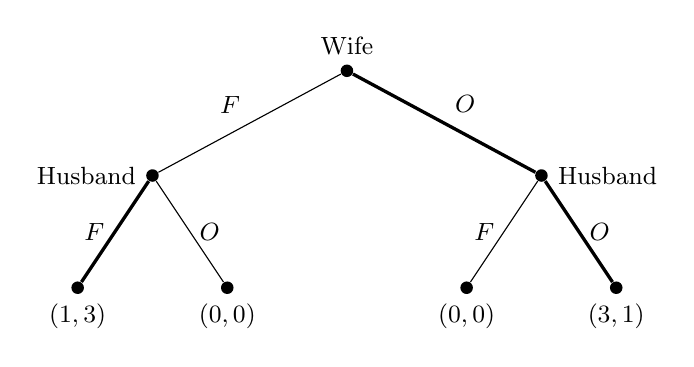
\begin{tikzpicture}[scale=0.95,dot/.style={circle,fill,inner sep=1.6pt},every node/.style={font=\small}]
  \node[dot,label=above:{Wife}] (r) at (0,0) {};
  \node[dot,label=left:{Husband}] (a) at (-2.6,-1.4) {};
  \node[dot,label=right:{Husband}] (b) at (2.6,-1.4) {};
  \draw (r) -- node[above left] {$F$} (a);
  \draw[very thick] (r) -- node[above right] {$O$} (b);
  \node[dot,label=below:{$(1,3)$}] (aa) at (-3.6,-2.9) {};
  \node[dot,label=below:{$(0,0)$}] (ab) at (-1.6,-2.9) {};
  \node[dot,label=below:{$(0,0)$}] (ba) at (1.6,-2.9) {};
  \node[dot,label=below:{$(3,1)$}] (bb) at (3.6,-2.9) {};
  \draw[very thick] (a) -- node[left] {$F$} (aa);
  \draw (a) -- node[right] {$O$} (ab);
  \draw (b) -- node[left] {$F$} (ba);
  \draw[very thick] (b) -- node[right] {$O$} (bb);
\end{tikzpicture}\\[2pt]
{\footnotesize Fig.~4.13 redrawn; thick branches = backward-induction choices.}
\end{center}

\textbf{(a) The husband's best replies.}
\begin{align*}
  \text{after } F:&\quad u_H(F,F) = 3 > 0 = u_H(F,O) \ \Rightarrow\ F;\\
  \text{after } O:&\quad u_H(O,O) = 1 > 0 = u_H(O,F) \ \Rightarrow\ O .
\end{align*}
The husband copies the wife: $s_H^* = FO$.

\textbf{(b) The wife's action and the SPE.} Replacing each husband node by his reply,
\[
  u_W(F, s_H^*) = u_W(F,F) = 1 \;<\; 3 = u_W(O,O) = u_W(O, s_H^*),
\]
so the wife chooses $O$. The subgame-perfect equilibrium is
\[
  (s_W^*, s_H^*) = (O,\ (F \text{ after } F,\ O \text{ after } O)) = (O, FO),
\]
with outcome $(O,O)$ and payoffs $(3,1)$. It is unique: both comparisons are strict.

\textbf{Normal form and Nash equilibria that are not subgame perfect.}
\begin{center}
\begin{tabular}{r|c|c|c|c|}
\multicolumn{1}{r}{} & \multicolumn{1}{c}{$FF$} & \multicolumn{1}{c}{$FO$} &
\multicolumn{1}{c}{$OF$} & \multicolumn{1}{c}{$OO$}\\ \cline{2-5}
$F$ & $\br{1},\ \br{3}$ & $1,\ \br{3}$ & $\br{0},\ 0$ & $0,\ 0$ \\ \cline{2-5}
$O$ & $0,\ 0$ & $\br{3},\ \br{1}$ & $\br{0},\ 0$ & $\br{3},\ \br{1}$ \\ \cline{2-5}
\end{tabular}
\end{center}
Underlined payoffs are best replies. The pure Nash equilibria are $(F, FF)$, $(O, FO)$ and $(O, OO)$.
Only $(O, FO)$ is subgame perfect. $(F, FF)$ rests on the husband's threat to go to Football even
after the wife chooses Opera (payoff $0$ for him, against $1$ from Opera), and $(O, OO)$ on his threat to
go to Opera even after Football (payoff $0$ against $3$): neither threat is a best reply in its subgame, so
neither is credible.

\textbf{(c) Comparison.} The simultaneous game has two pure equilibria, $(F,F)$ with $(1,3)$ and $(O,O)$
with $(3,1)$, and a mixed one (Lecture~3, slides~27--34); which is played is undetermined. In the sequential
game the husband observes the wife and copies her, so the wife can pick her favorite: the unique SPE
outcome is $(O,O)$, her best equilibrium of the simultaneous game. Moving first is an advantage here: the wife
earns $3$ instead of $1$ or the mixed-equilibrium payoff. The Football outcome $(F,F)$ is a Nash
equilibrium of the sequential game too, but only through a non-credible threat.

\interp The first-mover advantage comes from commitment: once the wife has moved, the husband
can only respond, and responding means coordinating on her choice. If the husband moved first the
opposite outcome would arise. The advantage depends on the \emph{coordination} structure: in the
prisoner's dilemma (item 3) moving first was worth nothing.

\verify \texttt{check\_L03.py} runs backward induction on the tree (the unique solution is path
$O$, $O$ with payoffs $(3,1)$), enumerates the pure Nash equilibria of the $2\times4$ normal form
and of the simultaneous game, and checks that exactly one of the three is a backward-induction profile.
Output line: \texttt{munoz-garcia-4-4: SPE (O, FO); pure NE (F,FF), (O,FO), (O,OO)}.
\emph{Comparison with \MG{}'s answer} (pp.~163--165): it agrees on all three parts, giving
$\mathrm{SPNE} = \{\text{Opera}, (\text{Football}, \text{Opera})\}$ with the husband's reply in
Subgame~2 (after Football) first and Subgame~3 (after Opera) second, and it states that the
husband moving first would reverse the outcome. The book does not list the non-subgame-perfect Nash equilibria.

\mistakes
\begin{itemize}
  \item Answering (a) as printed (the wife's best reply to the husband's action): the husband observes the wife,
  not the reverse.
  \item Writing the SPE as the outcome $(O,O)$ or as ``wife Opera, husband Opera'': the husband's strategy
  must also say what he does after Football, so the SPE is $(O, FO)$.
  \item Concluding that $(F,F)$ cannot be an equilibrium of the sequential game: it is a Nash equilibrium
  (sustained by $FF$), just not a subgame-perfect one.
\end{itemize}

\answer{(a) The husband replies Football after Football ($3 > 0$) and Opera after Opera ($1 > 0$).
(b) The wife chooses Opera ($3 > 1$); SPE $= (O, (F,O))$, outcome $(O,O)$, payoffs $(3,1)$.
Nash equilibria: $(F,FF)$, $(O,FO)$, $(O,OO)$; only $(O,FO)$ is subgame perfect.
(c) Yes: the simultaneous game has two pure equilibria and a mixed one; the sequential game's unique
SPE outcome is the wife's preferred one, $(O,O)$ (first-mover advantage).}
\end{exsol}
